% Standalone figure: 3D Active Vision Scenario
% Two scenario types: flat ground plane (green) and cylindrical object (red).
% Landscape golden-ratio aspect: width/height = 1.618
%
% Compile:        pdflatex fig_scenario.tex
% Include in paper: 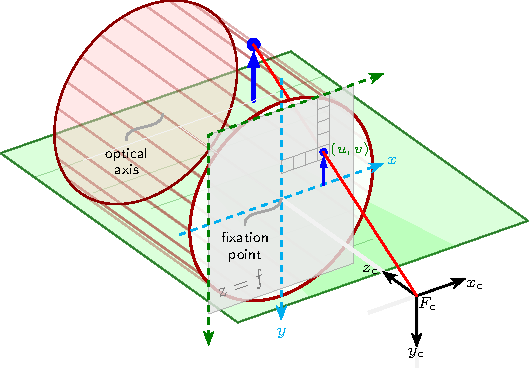
\includegraphics{fig_scenario}
%
% Note: the golden-ratio bounding box is enforced by extending the TikZ bbox
% in 2D after the 3D scope, so recompiling preserves the aspect ratio.
\documentclass[border=10pt,multi,tikz]{standalone}
\usepackage{tikz-3dplot}
\usetikzlibrary{calc,arrows.meta,positioning,backgrounds,shadings,fadings}

\begin{document}

\tdplotsetmaincoords{-60}{-35}

\begin{tikzpicture}
  % All global styles live on the outer tikzpicture (no tdplot_main_coords
  % here so we can escape to 2D at the end for the aspect-ratio fix).
  [
    >=Stealth,
    my dashed/.style={dashed, thick, ->, shorten >=-15pt, shorten <=-15pt,
        every node/.append style={font=\footnotesize}},
    my box/.style={thin, gray!70},
    my blue/.style={blue, line cap=round,
        -{Triangle[width=3*#1]}, line width=#1,
        shorten >=#1*1.75pt,
        every node/.append style={fill, circle, inner sep=0pt,
            minimum size=#1*3.5pt, anchor=center, outer sep=0pt}},
    my label/.append style={midway, font=\scriptsize},
    my vectors/.style={green!50!black,
        {Stealth[scale=.75]}-{Stealth[scale=.75]}},
    my red/.style={thick, red, line cap=round},
    my grey/.style={gray!70},
    description/.style={draw=gray!70, thick, line cap=round,
        every node/.style={align=center, font=\scriptsize\sffamily,
            anchor=north}},
    ground/.style={green!60!black, fill opacity=0.35, draw opacity=0.7,
        draw=green!40!black, line width=0.6pt},
    cylinder body/.style={red!70!black, fill opacity=0.55,
        draw=red!50!black, line width=0.8pt},
  ]

  % ==================================================================
  % ALL 3-D CONTENT inside this scope; closing it returns us to 2D.
  % ==================================================================
  \begin{scope}[tdplot_main_coords]

    % ----------------------------------------------------------------
    % GROUND PLANE (z = 0)  –  green with perspective grid
    % ----------------------------------------------------------------
    \begin{scope}[on background layer]
      \path [ground, fill=green!40!white]
          (-3,1,0) -- (3,1,0) -- (3,8,0) -- (-3,8,0) -- cycle;
      % Lighter inner quad (closer to camera) for depth cue
      \path [fill=green!80!white, fill opacity=0.18]
          (-1.5,1,0) -- (1.5,1,0) -- (.8,5,0) -- (-.8,5,0) -- cycle;
      % Horizontal grid lines converging with depth
      \foreach \yy in {2,3,...,7} {
        \pgfmathsetmacro\xmax{0.5*\yy-0.5}
        \draw [green!50!black, opacity=0.30, thin]
            (-\xmax,\yy,0) -- (\xmax,\yy,0);
      }
      % Radial grid lines for perspective
      \foreach \xx in {-2,-1,0,1,2} {
        \draw [green!50!black, opacity=0.25, thin]
            (\xx,1,0) -- (\xx*2.5,8,0);
      }
      \draw [green!40!black, opacity=0.6, thin]
          (-3,1,0) -- (3,1,0) -- (3,8,0) -- (-3,8,0) -- cycle;
    \end{scope}

    % ----------------------------------------------------------------
    % RED CYLINDER  –  represents a 3-D object in the scene
    % ----------------------------------------------------------------
    \def\Cx{1.8}  \def\Cy{5.5}  \def\Ch{1.6}  \def\Cr{0.35}

    \begin{scope}[on background layer]
      % Main face (lit)
      \path [cylinder body, fill=red!50!white]
          (\Cx-\Cr,\Cy,0) -- (\Cx-\Cr,\Cy,\Ch)
          -- (\Cx+\Cr,\Cy,\Ch) -- (\Cx+\Cr,\Cy,0) -- cycle;
      % Shadow face (darker right edge)
      \path [fill=red!70!black, fill opacity=0.45, draw=none]
          (\Cx+\Cr,\Cy,0) -- (\Cx+\Cr,\Cy,\Ch)
          -- (\Cx+\Cr,\Cy+0.01,\Ch) -- (\Cx+\Cr,\Cy+0.01,0) -- cycle;
    \end{scope}
    % Top cap (bright)
    \draw [fill=red!40!white, fill opacity=0.65,
           draw=red!50!black, line width=0.8pt]
        (\Cx-\Cr,\Cy,\Ch) -- (\Cx+\Cr,\Cy,\Ch) -- cycle;
    \draw [red!60!black, line width=1pt]
        (\Cx-\Cr,\Cy,\Ch) -- (\Cx+\Cr,\Cy,\Ch);
    % Vertical edges
    \draw [cylinder body] (\Cx-\Cr,\Cy,0) -- (\Cx-\Cr,\Cy,\Ch);
    \draw [cylinder body] (\Cx+\Cr,\Cy,0) -- (\Cx+\Cr,\Cy,\Ch);
    % Bottom edge
    \draw [cylinder body] (\Cx-\Cr,\Cy,0) -- (\Cx+\Cr,\Cy,0);
    % Label
    \node [red!70!black, font=\scriptsize\sffamily, anchor=west]
        at (\Cx+\Cr+0.1,\Cy,\Ch*0.5) {3-D object};

    % ----------------------------------------------------------------
    % CAMERA / IMAGE-PLANE CONTENT  (from original draft, unchanged)
    % ----------------------------------------------------------------
    \draw [my grey] (0,4,0) -- (0,7,0) (-2,7,0) -- (2,7,0);
    \coordinate (o) at (0,0,0);

    % Focal plane
    \path [draw=gray!70, text=gray, fill=gray!20, opacity=0.8,
           text opacity=1]
        (-1.5,4,1.75) coordinate (a) --
        ++(0,0,-3.5)  coordinate (b) --
        ++(3,0,0)     coordinate (c) --
        ++(0,0,3.5)   coordinate (d) -- cycle
        node [pos=.95, above, sloped, anchor=south west] {$z=f$};

    \draw [my grey]
        (-2,0,0) -- (2,0,0)
        (0,0,0) -- (0,4,0)
        (0,0,0) -- (0,0,2);

    % Camera frame axes
    \draw [thick, ->,
           every node/.style={font=\footnotesize, inner sep=0pt}]
        (o) node [anchor=north west] {$F_c$}
        (o) edge node [pos=1, anchor=north east] {$z_c$} ++(0,1,0)
            edge node [pos=1, anchor=north]      {$y_c$} ++(0,0,1)
            -- ++(1,0,0) node [anchor=north west] {$x_c$};

    % Pixel grid
    \draw [my box] (o) ++(0,4,-.5) coordinate (p1)
        -- ++(1,0,0) coordinate (p2)
        -- ++(0,0,-1.25) coordinate (p3);
    \foreach \i in {0,1,...,4}
        \draw [my box] (p1) ++(\i*.25,0,0) -- ++(0,0,-.25);
    \foreach \i in {0,1,...,5}
        \draw [my box] (p2) ++(0,0,-\i*.25) -- ++(-.25,0,0);
    \draw [my box] (p1) ++(0,0,-.25) -- ++(.75,0,0) -- ++(0,0,-1);

    % Image-plane axes (cyan dashed)
    \draw [my dashed, cyan] ($(b)!1/2!(c)$) -- ($(d)!1/2!(a)$)
        node [below=15pt, anchor=north] {$y$};
    \draw [my dashed, cyan] ($(b)!1/2!(a)$) -- ($(d)!1/2!(c)$)
        node [above right=17pt, anchor=north west] {$x$};

    % Pixel coordinate vectors
    \draw [my dashed, green!50!black, <->]
        (a) node [below=15pt, anchor=north] {$v$} --
        (b) -- (c) node [above right=17pt, anchor=north west] {$u$};
    \path [green!50!black,
           every node/.style={font=\scriptsize, inner sep=0pt}]
        (p2) node [above right, anchor=south west] {$(u,v)$};

    \path (p2) ++(-.125,0,0) coordinate (q2)
              ++(0,0,-.125)  coordinate (r2);

    % Ray from pixel to scene
    \draw [my blue=1]
        ($(0,4,0)+($(q2)-(p1)$)$) coordinate (s2) -- (r2) node (d1) {};

    \scoped[on background layer]{
      \draw [my blue=1.75]
          ($($1.75*($(s2)-(0,4,0)$)$)+(0,7,0)$) --
          ++($1.75*($(r2)-(s2)$)$)
          node (d2)
              [label={[label distance=-50pt]above:
                  {$P=(R\cdot\cos\theta,\,R\cdot\sin\theta,\,Z)$}}] {};
    }

    % u, v image vectors
    \draw [my vectors] (0,4,.1) -- ($(s2)+(0,0,.1)$)
        node [below, my label, sloped] {$\vec{u}$};
    \draw [my vectors] (-.1,4,0) -- ($(q2)-(s2)+(-.1,4,0)$)
        node [left, my label] {$\vec{v}$};

    % Optical ray in world space
    \draw [my red] (o) -- (d1.center);
    \scoped[on background layer]{
        \draw [my red] (d1.center) -- (d2.center);
    }

    % Annotation callouts
    \path [description]
        (0,4,0)   [out=-95, in=95] to (-.75,4,.25)
            node {fixation\\point}
        (0,6.5,0) [out=-95, in=95] to (-.75,6.5,.25)
            node {optical\\axis};

  \end{scope} % end tdplot_main_coords scope  ← we are now in 2D

  % ==================================================================
  % GOLDEN-RATIO BOUNDING-BOX EXTENSION (pure 2D, no 3D transform)
  %
  % The 3D content compiles to ~300×240 pt (excl. border).  To reach
  % a 1:φ (=1:1.618) landscape ratio with the 10 pt border:
  %   target_content_W = (240+20)×1.618 − 20 ≈ 400.7 pt
  %   extra per side   = (400.7−300)/2     ≈  50.3 pt
  %
  % We extend with invisible \path points so standalone auto-crops
  % to the correct bounding box.  No recompilation needed.
  % ==================================================================
  \path ([xshift=-50.34pt]current bounding box.south west)
        ([xshift=+50.34pt]current bounding box.north east);

\end{tikzpicture}

\end{document}
